% Options for packages loaded elsewhere
\PassOptionsToPackage{unicode}{hyperref}
\PassOptionsToPackage{hyphens}{url}
\documentclass[
  ignorenonframetext,
]{beamer}
\newif\ifbibliography
\usepackage{pgfpages}
\setbeamertemplate{caption}[numbered]
\setbeamertemplate{caption label separator}{: }
\setbeamercolor{caption name}{fg=normal text.fg}
\beamertemplatenavigationsymbolsempty
% remove section numbering
\setbeamertemplate{part page}{
  \centering
  \begin{beamercolorbox}[sep=16pt,center]{part title}
    \usebeamerfont{part title}\insertpart\par
  \end{beamercolorbox}
}
\setbeamertemplate{section page}{
  \centering
  \begin{beamercolorbox}[sep=12pt,center]{section title}
    \usebeamerfont{section title}\insertsection\par
  \end{beamercolorbox}
}
\setbeamertemplate{subsection page}{
  \centering
  \begin{beamercolorbox}[sep=8pt,center]{subsection title}
    \usebeamerfont{subsection title}\insertsubsection\par
  \end{beamercolorbox}
}
% Prevent slide breaks in the middle of a paragraph
\widowpenalties 1 10000
\raggedbottom
\AtBeginPart{
  \frame{\partpage}
}
\AtBeginSection{
  \ifbibliography
  \else
    \frame{\sectionpage}
  \fi
}
\AtBeginSubsection{
  \frame{\subsectionpage}
}
\usepackage{iftex}
\ifPDFTeX
  \usepackage[T1]{fontenc}
  \usepackage[utf8]{inputenc}
  \usepackage{textcomp} % provide euro and other symbols
\else % if luatex or xetex
  \usepackage{unicode-math} % this also loads fontspec
  \defaultfontfeatures{Scale=MatchLowercase}
  \defaultfontfeatures[\rmfamily]{Ligatures=TeX,Scale=1}
\fi
\usepackage{lmodern}
\ifPDFTeX\else
  % xetex/luatex font selection
\fi
% Use upquote if available, for straight quotes in verbatim environments
\IfFileExists{upquote.sty}{\usepackage{upquote}}{}
\IfFileExists{microtype.sty}{% use microtype if available
  \usepackage[]{microtype}
  \UseMicrotypeSet[protrusion]{basicmath} % disable protrusion for tt fonts
}{}
\makeatletter
\@ifundefined{KOMAClassName}{% if non-KOMA class
  \IfFileExists{parskip.sty}{%
    \usepackage{parskip}
  }{% else
    \setlength{\parindent}{0pt}
    \setlength{\parskip}{6pt plus 2pt minus 1pt}}
}{% if KOMA class
  \KOMAoptions{parskip=half}}
\makeatother
\usepackage{longtable,booktabs,array}
\usepackage{caption}
\captionsetup[table]{skip=6pt}
\newcounter{none} % for unnumbered tables
\usepackage{calc} % for calculating minipage widths
\usepackage{caption}
% Make caption package work with longtable
\makeatletter
\def\fnum@table{\tablename~\thetable}
\makeatother
\usepackage{graphicx}
\makeatletter
\newsavebox\pandoc@box
\newcommand*\pandocbounded[1]{% scales image to fit in text height/width
  \sbox\pandoc@box{#1}%
  \Gscale@div\@tempa{\textheight}{\dimexpr\ht\pandoc@box+\dp\pandoc@box\relax}%
  \Gscale@div\@tempb{\linewidth}{\wd\pandoc@box}%
  \ifdim\@tempb\p@<\@tempa\p@\let\@tempa\@tempb\fi% select the smaller of both
  \ifdim\@tempa\p@<\p@\scalebox{\@tempa}{\usebox\pandoc@box}%
  \else\usebox{\pandoc@box}%
  \fi%
}
% Set default figure placement to htbp
\def\fps@figure{htbp}
\makeatother
\setlength{\emergencystretch}{3em} % prevent overfull lines
\providecommand{\tightlist}{%
  \setlength{\itemsep}{0pt}\setlength{\parskip}{0pt}}
% Manuscript macro/package fallbacks (newcommand -> providecommand).
% Core mathematical packages
\usepackage{amsmath,amssymb,amsthm}
\usepackage{mathtools}
% Permit bibliography and theorem prose to break without overfull boxes.
% Algorithm formatting
% Tables
\usepackage{booktabs}
\usepackage{multirow}
% Graphics
% Cross-referencing with smart naming
% Configure cleveref for custom environments
% Theorem environments with consistent numbering
% Code listings used by supplementary implementation examples
\usepackage{listings}
\lstset{basicstyle=\ttfamily\small,breaklines=true,columns=fullflexible}
% End of theorem environment declarations
% Math operators
\DeclareMathOperator*{\argmax}{arg\,max}
\DeclareMathOperator*{\argmin}{arg\,min}
\DeclareMathOperator{\sign}{sign}
\DeclareMathOperator{\KL}{KL}
\DeclareMathOperator{\Tr}{Tr}
% Custom commands for notation consistency
\providecommand{\calA}{\mathcal{A}}
\providecommand{\calB}{\mathcal{B}}
\providecommand{\calC}{\mathcal{C}}
\providecommand{\calD}{\mathcal{D}}
\providecommand{\calF}{\mathcal{F}}
\providecommand{\calG}{\mathcal{G}}
\providecommand{\calH}{\mathcal{H}}
\providecommand{\calI}{\mathcal{I}}
\providecommand{\calM}{\mathcal{M}}
\providecommand{\calO}{\mathcal{O}}
\providecommand{\calP}{\mathcal{P}}
\providecommand{\calS}{\mathcal{S}}
\providecommand{\calT}{\mathcal{T}}
\providecommand{\calW}{\mathcal{W}}
% Note: \Phi is a standard LaTeX command, do not redefine
% Trust notation
\providecommand{\trust}[2]{\mathcal{T}_{#1 \to #2}}
\providecommand{\trustt}[3]{\mathcal{T}_{#1 \to #2}^{#3}}
% Belief notation
\providecommand{\belief}[2]{\mathcal{B}_{#1}(#2)}
\providecommand{\belieft}[3]{\mathcal{B}_{#1}^{#2}(#3)}
% Cognitive state
\providecommand{\cogstate}[1]{\sigma_{#1}}
% Attack notation
\providecommand{\attack}[1]{\mathcal{A}_{#1}}
\providecommand{\adversary}[1]{\Omega_{#1}}
% Defense notation
\providecommand{\firewall}{\mathcal{F}}
\providecommand{\sandbox}{\mathcal{S}_{box}}
% Probability and expectation
\providecommand{\E}{\mathbb{E}}
\providecommand{\Prob}{\mathbb{P}}
\providecommand{\indicator}{\mathbb{1}}
% QED symbol
\providecommand{\qedsymbol}{$\blacksquare$}
% Page Layout (Slightly smaller margins)
% Hyperlink Styling
% List of Figures and List of Tables in TOC

% Slide layout defaults for warning-clean scientific decks.
\usepackage{etoolbox}
\IfFileExists{xurl.sty}{\usepackage{xurl}}{}
\IfFileExists{seqsplit.sty}{\usepackage{seqsplit}}{\newcommand{\seqsplit}[1]{#1}}
\protected\def\breakseq#1{\seqsplit{#1}}
\protected\def\breaktt#1{\begingroup\ttfamily\seqsplit{#1}\endgroup}
\setlength{\emergencystretch}{6em}
\tolerance=5000
\hbadness=10000
\hfuzz=1pt
\setlength{\tabcolsep}{2pt}
\AtBeginEnvironment{longtable}{\tiny\renewcommand{\arraystretch}{0.86}\setlength{\tabcolsep}{1pt}}
\AtBeginEnvironment{tabular}{\tiny\renewcommand{\arraystretch}{0.86}\setlength{\tabcolsep}{1pt}}
\AtBeginEnvironment{equation}{\tiny}
\AtBeginEnvironment{equation*}{\tiny}
\AtBeginEnvironment{align}{\tiny}
\AtBeginEnvironment{align*}{\tiny}
\AtBeginEnvironment{itemize}{\footnotesize}
\AtBeginEnvironment{enumerate}{\footnotesize}
\AtBeginEnvironment{description}{\footnotesize}
\setbeamerfont{caption}{size=\tiny}
\setbeamerfont{caption name}{size=\tiny}
\setbeamerfont{normal text}{size=\small}
\setbeamerfont{frametitle}{size=\small}
\setbeamerfont{section title}{size=\footnotesize}
\setbeamerfont{subsection title}{size=\footnotesize}
\setbeamertemplate{section page}{%
  \centering
  \begin{beamercolorbox}[sep=12pt,center,wd=\paperwidth]{section title}
    \parbox{0.86\paperwidth}{\centering\usebeamerfont{section title}\insertsection\par}
  \end{beamercolorbox}
}
\setbeamertemplate{subsection page}{%
  \centering
  \begin{beamercolorbox}[sep=8pt,center,wd=\paperwidth]{subsection title}
    \parbox{0.86\paperwidth}{\centering\usebeamerfont{subsection title}\insertsubsection\par}
  \end{beamercolorbox}
}
\setlength{\abovecaptionskip}{2pt}
\setlength{\belowcaptionskip}{0pt}

% Natbib and cross-reference fallbacks — slides don't load natbib
% or cleveref, but combined-PDF manuscript prose may emit these
% commands. The fallback renders citations as a bracketed key list
% and cross-references as detokenized labels so slides don't fail on
% undefined control sequences or raw underscores. \providecommand is
% a no-op if packages load later.
\providecommand{\citep}[1]{[#1]}
\providecommand{\citet}[1]{#1}
\providecommand{\citealp}[1]{#1}
\providecommand{\citeauthor}[1]{#1}
\providecommand{\citeyear}[1]{#1}
\providecommand{\cref}[1]{\texttt{\detokenize{#1}}}
\providecommand{\Cref}[1]{\texttt{\detokenize{#1}}}
\providecommand{\crefrange}[2]{\texttt{\detokenize{#1}}--\texttt{\detokenize{#2}}}
\providecommand{\Crefrange}[2]{\texttt{\detokenize{#1}}--\texttt{\detokenize{#2}}}
\providecommand{\paragraph}[1]{\textbf{#1}\ }

% Additional theorem-like environments from manuscript preamble.
\newtheorem{observation}{Observation}
\newtheorem{formalization}{Formalization}
\newtheorem{principle}{Principle}

\newtheorem{proposition}{Proposition}
\newtheorem{hypothesis}{Hypothesis}
\newtheorem{remark}[theorem]{Remark}
\newtheorem{axiom}{Axiom}
\newtheorem{property}{Property}
\usepackage{bookmark}
\IfFileExists{xurl.sty}{\usepackage{xurl}}{} % add URL line breaks if available
\urlstyle{same}
% fallback for those not using the hyperref driver hyperxmp:
\makeatletter
\@ifundefined{xmpquote}{\newcommand{\xmpquote}[1]{#1}}{}
\makeatother
\hypersetup{
  hidelinks,
  pdfcreator={LaTeX via pandoc}}

\author{\texorpdfstring{}{}}
\date{}

\begin{document}

\begin{frame}
\newpage
\end{frame}

\section{Detection Methods: Anomaly Detection, ROC Analysis, and
Provenance Tracking}\label{sec:detection-methods}

\begin{frame}[allowframebreaks]{Detection Methods: Anomaly Detection,
ROC Analysis, and Provenance Tracking}
This section presents the formal foundations for cognitive attack
detection. We define anomaly detection metrics
(\cref{sec:anomaly-detection}), ROC curve framework
(\cref{sec:roc-analysis}), multi-detector fusion theory
(\cref{sec:detector-fusion}), online vs.~batch trade-offs
(\cref{sec:online-batch}), false positive mitigation strategies
(\cref{sec:fp-mitigation}), provenance analysis (\cref{sec:provenance}),
and real-time monitoring architecture (\cref{sec:monitoring}).

\end{frame}

\begin{frame}[allowframebreaks]{Detection Methods: Anomaly Detection,
ROC Analysis, and Provenance Tracking}
\begin{quote}
\textbf{Note}: For algorithm implementations and empirical performance
results, see Part 2 of this series \cite{friedman2026cogsec2}.
Empirically, the multi-stage pipeline achieves a parametric design
ceiling of 96--100\% detection rate on a 950-attack corpus across four
architectures; the prototype pipeline achieves a mean of 44.8\% {[}95\%
CI: 43.2\%, 46.4\%{]} across 30 seeds. Part 2 reports no measured
per-\(\Omega\)-class detection rates: the corpus carries a design-level
\(\Omega\) classification rather than a runtime label, so per-class
rates are not evaluated.
\end{quote}
\end{frame}

\subsection{Anomaly Detection}\label{sec:anomaly-detection}

\begin{frame}[allowframebreaks]{Cognitive Drift Scoring}
\protect\phantomsection\label{cognitive-drift-scoring}
\begin{definition}[Drift Score]
\label{def:drift-score}
The cognitive drift score measures belief distribution change over time:
\begin{equation}
\label{eq:drift-score}
S_{\text{drift}}(t) = D_{\text{KL}}(\mathcal{B}_i^t \| \mathcal{B}_i^{t-w}) + \lambda \cdot \max_\phi |\Delta \mathcal{B}_i(\phi)|
\end{equation}
\end{definition}

\end{frame}

\begin{frame}[allowframebreaks]{Cognitive Drift Scoring}
\begin{table}[htbp]
\centering
\caption{Drift score components and detection targets.}
\label{tab:drift-components}
\begin{tabular}{@{}llp{5cm}@{}}
\toprule
Component & Weight & Detection Target \\
\midrule
KL divergence & 1.0 & Gradual distribution shift \\
Max delta & $\lambda$ & Sudden belief injection \\
\bottomrule
\end{tabular}
\end{table}

\begin{property}[Drift Detection Threshold]
\label{prop:drift-threshold}
For normally distributed baseline drift, the threshold $\theta = \mu_{\text{baseline}} + k \cdot \sigma_{\text{baseline}}$ with $k = 3$ provides $99.7\%$ confidence under the null hypothesis of no attack.
\end{property}
\end{frame}

\begin{frame}[allowframebreaks]{Behavioral Deviation Scoring}
\protect\phantomsection\label{behavioral-deviation-scoring}
\begin{definition}[Deviation Score]
\label{def:deviation-score}
The behavioral deviation score aggregates normalized feature anomalies:
\begin{equation}
\label{eq:deviation-score}
S_{\text{dev}}(a_i, t) = \sum_{k=1}^K w_k \cdot \frac{|f_k(\sigma_i^t) - \mu_k|}{\sigma_k}
\end{equation}
where $f_k$ are feature extractors and $(w_k, \mu_k, \sigma_k)$ are learned parameters.
\end{definition}
\end{frame}

\begin{frame}[allowframebreaks]{Ensemble Detection}
\protect\phantomsection\label{ensemble-detection}
\begin{definition}[Ensemble Detector]
\label{def:ensemble-detector}
Combines multiple detector scores via learned fusion:
\begin{equation}
\label{eq:ensemble-detector}
P(\text{attack} \mid \mathbf{S}) = \sigma\left(\sum_d w_d \cdot S_d - b\right)
\end{equation}
where $\sigma$ is the sigmoid function and weights $(w_d, b)$ are learned from labeled examples.
\end{definition}
\end{frame}

\subsection{ROC Curve Analysis}\label{sec:roc-analysis}

\begin{frame}[allowframebreaks]{ROC Curve Analysis}
\begin{figure}
\centering
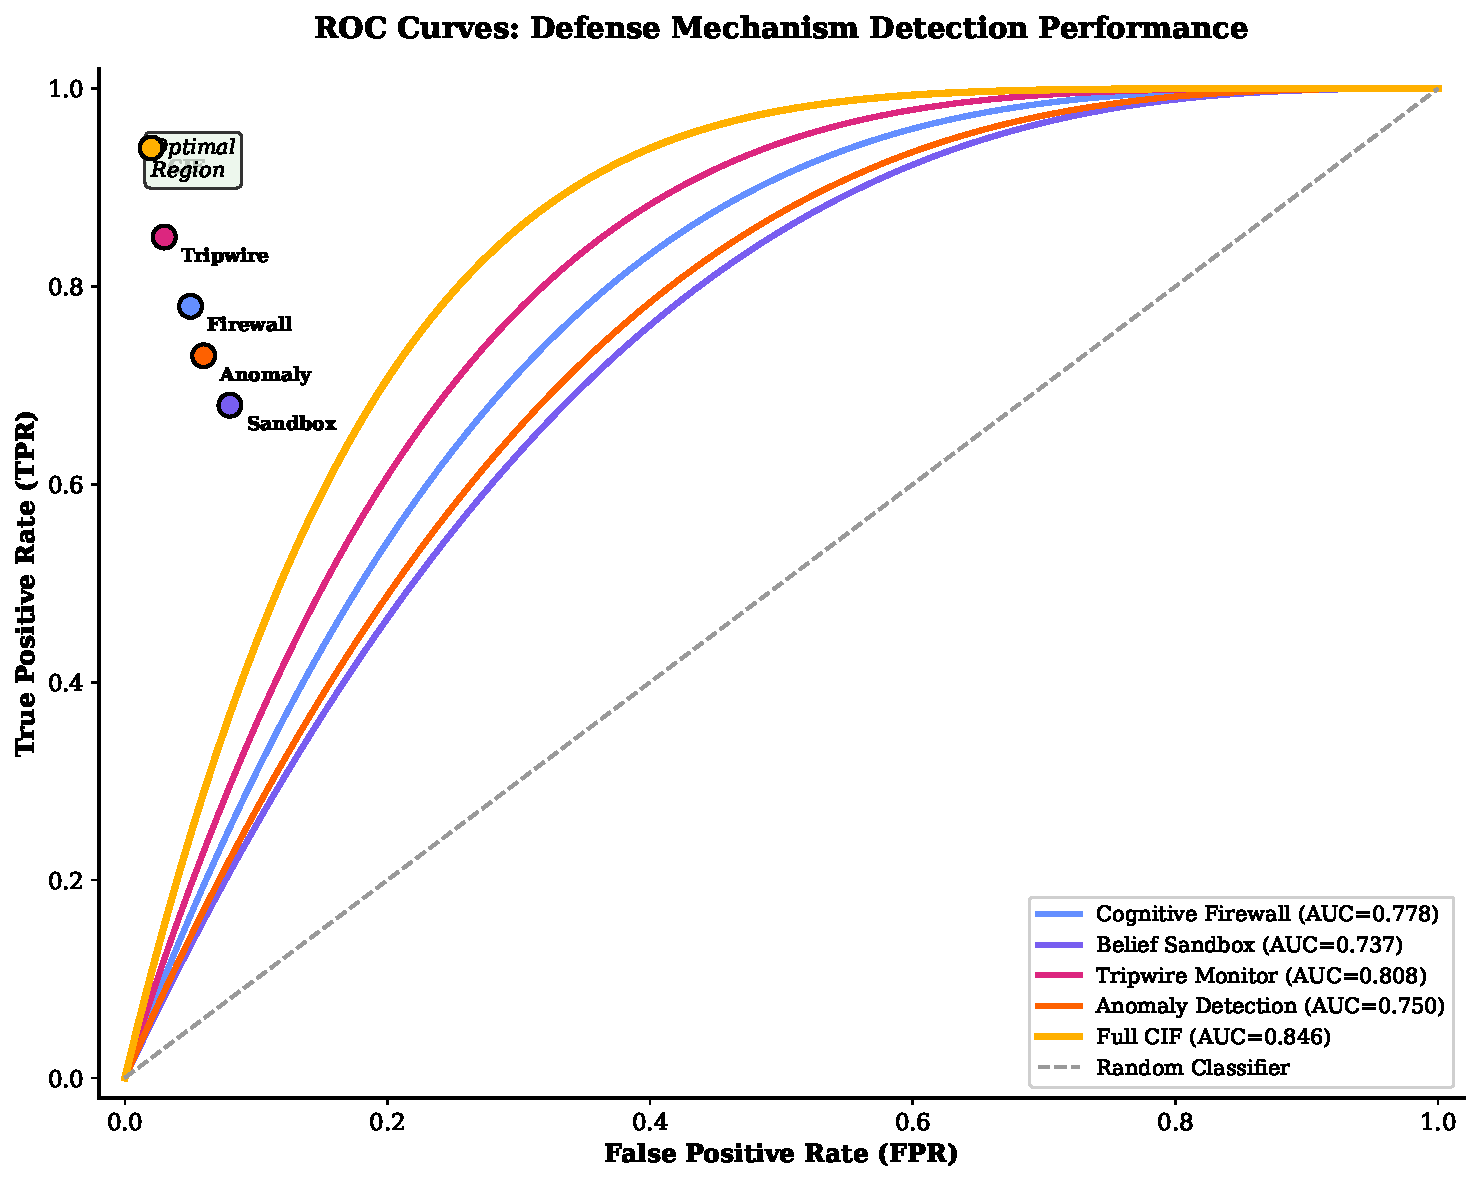
\includegraphics[width=0.85\linewidth,height=0.40\textheight,keepaspectratio,alt={Receiver Operating Characteristic (ROC) curves for CIF detection across attack categories (illustrative/schematic operating points under the Neyman-Pearson framework; the sandbox/tripwire/anomaly/full-CIF curves are labeled Theoretical, not empirical measurements, whereas the Cognitive Firewall curve is the Part-1 curve measured over the module's small test corpus --- measured eval curves are reported in Part 2).}]{../figures/roc_curves.pdf}
\caption{Receiver Operating Characteristic (ROC) curves for CIF
detection across attack categories (illustrative/schematic operating
points under the Neyman-Pearson framework; the
sandbox/tripwire/anomaly/full-CIF curves are labeled Theoretical, not
empirical measurements, whereas the Cognitive Firewall curve is the
Part-1 curve measured over the module's small test corpus --- measured
eval curves are reported in Part 2).}\label{fig:roc-curves}
\end{figure}
\end{frame}

\begin{frame}[allowframebreaks]{Receiver Operating Characteristic
Framework}
\protect\phantomsection\label{receiver-operating-characteristic-framework}
\begin{definition}[ROC Curve]
\label{def:roc-curve}
For detector $D$ with threshold $\tau$:
\begin{equation}
\label{eq:roc-curve}
\text{ROC}(D) = \{(\text{FPR}(\tau), \text{TPR}(\tau)) : \tau \in [0, 1]\}
\end{equation}
where the rates are defined as:
\begin{align}
\label{eq:tpr}
\text{TPR}(\tau) &= P(D(x) > \tau \mid x \in \mathcal{A}_{\text{attack}}) \\
\label{eq:fpr}
\text{FPR}(\tau) &= P(D(x) > \tau \mid x \in \mathcal{X}_{\text{benign}})
\end{align}
\end{definition}

\begin{definition}[Area Under Curve]
\label{def:auc}
\begin{equation}
\label{eq:auc}
\text{AUC}(D) = \int_0^1 \text{TPR}(\text{FPR}^{-1}(t)) \, dt
\end{equation}
\end{definition}

\end{frame}

\begin{frame}[allowframebreaks]{Receiver Operating Characteristic
Framework}
\begin{table}[htbp]
\centering
\caption{AUC interpretation scale.}
\label{tab:auc-interpretation}
\begin{tabular}{@{}ll@{}}
\toprule
AUC Range & Interpretation \\
\midrule
$0.5$ & Random classifier \\
$0.7$--$0.8$ & Acceptable discrimination \\
$0.8$--$0.9$ & Good discrimination \\
$0.9$--$1.0$ & Excellent discrimination \\
\bottomrule
\end{tabular}
\end{table}
\end{frame}

\begin{frame}[allowframebreaks]{Confidence Intervals for AUC}
\protect\phantomsection\label{confidence-intervals-for-auc}
\begin{definition}[AUC Confidence Interval]
\label{def:auc-ci}
Using DeLong's method:
\begin{equation}
\label{eq:auc-ci}
\text{CI}_{95\%}(\text{AUC}) = \text{AUC} \pm 1.96 \cdot \sqrt{\text{Var}(\text{AUC})}
\end{equation}
where:
\begin{equation}
\label{eq:auc-variance}
\text{Var}(\text{AUC}) = \frac{1}{n_a} \sum_{i=1}^{n_a} (V_1^i - \text{AUC})^2 + \frac{1}{n_b} \sum_{j=1}^{n_b} (V_0^j - \text{AUC})^2
\end{equation}
\end{definition}
\end{frame}

\subsection{Multi-Detector Fusion}\label{sec:detector-fusion}

\begin{frame}[allowframebreaks]{Fusion Strategies}
\protect\phantomsection\label{fusion-strategies}
\begin{definition}[Score-Level Fusion]
\label{def:score-fusion}
Weighted average of detector outputs:
\begin{equation}
\label{eq:score-fusion}
S_{\text{fused}} = \sum_{i=1}^k w_i \cdot S_i, \quad \sum_i w_i = 1
\end{equation}
\end{definition}

\begin{definition}[Decision-Level Fusion]
\label{def:decision-fusion}
Quorum voting on binary decisions:
\begin{equation}
\label{eq:decision-fusion}
D_{\text{fused}}(x) = \mathbb{1}\left[\sum_{i=1}^k \mathbb{1}[D_i(x) > \tau_i] \geq q\right]
\end{equation}
\end{definition}

\begin{definition}[Learned Fusion]
\label{def:learned-fusion}
Neural network combining scores:
\begin{equation}
\label{eq:learned-fusion}
S_{\text{fused}} = \text{MLP}(S_1, \ldots, S_k; \theta)
\end{equation}
\end{definition}
\end{frame}

\begin{frame}[allowframebreaks]{Diversity-Aware Fusion}
\protect\phantomsection\label{diversity-aware-fusion}
\begin{definition}[Detector Diversity]
\label{def:detector-diversity}
\begin{equation}
\label{eq:detector-diversity}
\text{Diversity}(D_i, D_j) = 1 - \frac{|\text{errors}(D_i) \cap \text{errors}(D_j)|}{|\text{errors}(D_i) \cup \text{errors}(D_j)|}
\end{equation}
\end{definition}

\begin{theorem}[Diversity Benefit]
\label{thm:diversity-benefit}
For detectors with error rates $e_1, \ldots, e_k$ and pairwise diversity $\delta_{ij}$:
\begin{equation}
\label{eq:diversity-benefit}
e_{\text{fusion}} \leq \prod_i e_i + (1 - \bar{\delta}) \cdot \max_i e_i
\end{equation}
where $\bar{\delta}$ is the average pairwise diversity.
\end{theorem}

\end{frame}

\begin{frame}[allowframebreaks]{Diversity-Aware Fusion}
\begin{proof}
When detectors make independent errors (high diversity), the fusion error is the product of individual errors. Error correlation reduces this benefit proportionally to $(1 - \bar{\delta})$.
\end{proof}
\end{frame}

\subsection{Online vs.~Batch Detection}\label{sec:online-batch}

\begin{frame}[allowframebreaks]{Comparison Framework}
\protect\phantomsection\label{comparison-framework}
\end{frame}

\begin{frame}[allowframebreaks]{Comparison Framework}
\begin{table}[htbp]
\centering
\caption{Online vs. batch detection trade-offs.}
\label{tab:online-batch-comparison}
\begin{tabular}{@{}lll@{}}
\toprule
Dimension & Online Detection & Batch Detection \\
\midrule
Latency & Low (ms) & High (minutes--hours) \\
Accuracy & Moderate & High \\
Context & Limited (window) & Full history \\
Compute & Streaming & Offline \\
Memory & $O(w)$ window & $O(n)$ full \\
Use Case & Real-time response & Forensics, tuning \\
\bottomrule
\end{tabular}
\end{table}
\end{frame}

\begin{frame}[allowframebreaks]{Streaming Detector Model}
\protect\phantomsection\label{streaming-detector-model}
\begin{definition}[Streaming Detector]
\label{def:streaming-detector}
Processes messages in real-time with bounded memory:
\begin{align}
\label{eq:streaming-output}
D_{\text{online}}(m_t) &= f(m_t, \text{state}_{t-1}) \\
\label{eq:streaming-state}
\text{state}_t &= g(\text{state}_{t-1}, m_t)
\end{align}
\end{definition}
\end{frame}

\begin{frame}[allowframebreaks]{Hybrid Detection Architecture}
\protect\phantomsection\label{hybrid-detection-architecture}
\begin{definition}[Hybrid Detection System]
\label{def:hybrid-detection}
Combines online and batch detection via feedback loop:
\begin{equation}
\label{eq:hybrid-architecture}
\text{Online Path}: m \xrightarrow{\text{filter}} s \xrightarrow{\text{decide}} r \xrightarrow{\text{log}} H
\end{equation}
\begin{equation}
\label{eq:hybrid-feedback}
\text{Batch Path}: H \xrightarrow{\text{analyze}} \text{patterns} \xrightarrow{\text{update}} \text{filters}
\end{equation}
\end{definition}
\end{frame}

\subsection{False Positive Mitigation}\label{sec:fp-mitigation}

\begin{frame}[allowframebreaks]{False Positive Mitigation}
\begin{figure}
\centering
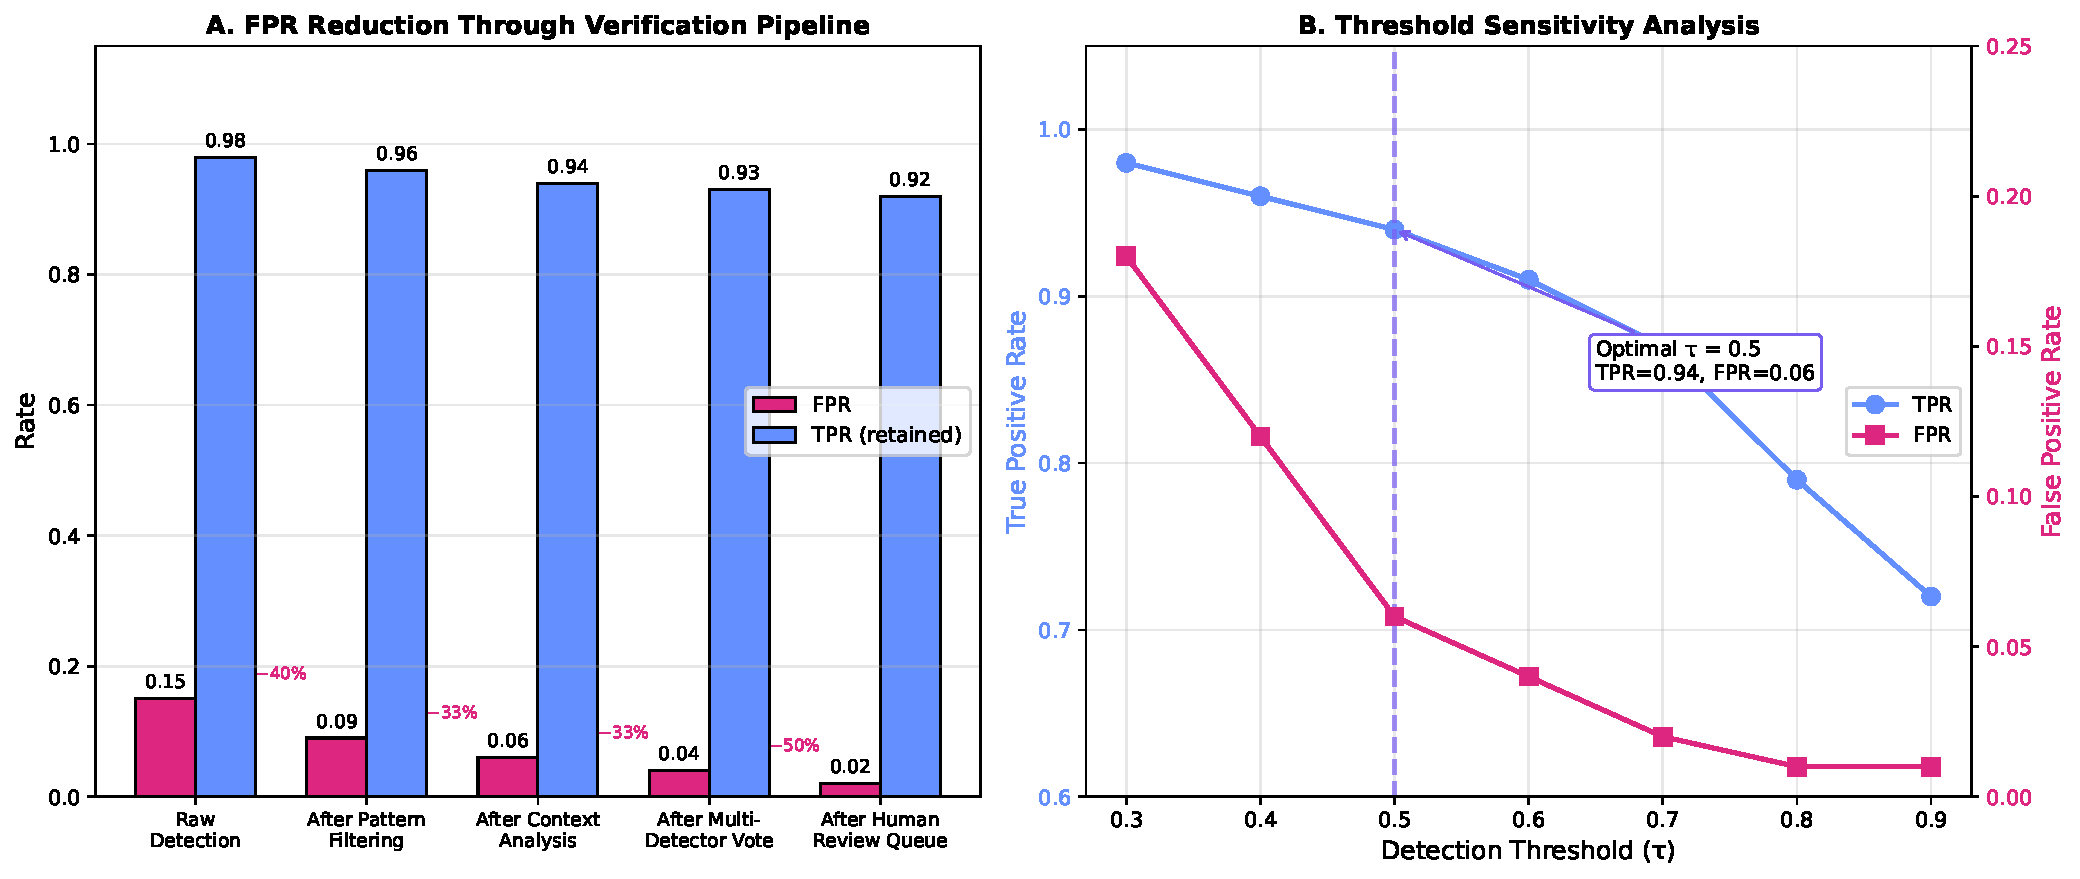
\includegraphics[width=0.8\linewidth,height=0.40\textheight,keepaspectratio,alt={False-positive mitigation (illustrative schematic): how the detection threshold and confidence calibration shape the false-positive / true-positive tradeoff.}]{../figures/fp_mitigation.pdf}
\caption{False-positive mitigation (illustrative schematic): how the
detection threshold and confidence calibration shape the false-positive
/ true-positive tradeoff.}\label{fig:fp-mitigation}
\end{figure}
\end{frame}

\begin{frame}[allowframebreaks]{Strategy 1: Confirmation Cascade}
\protect\phantomsection\label{strategy-1-confirmation-cascade}
\begin{definition}[Confirmation Cascade]
\label{def:confirmation-cascade}
Multi-stage verification before alerting:
\begin{equation}
\label{eq:cascade-decision}
\text{Action}(\text{confidence}) = \begin{cases}
\text{suppress} & \text{if } c < C_{\text{low}} \\
\text{stage-2} & \text{if } c \in [C_{\text{low}}, C_{\text{high}}) \\
\text{stage-3} & \text{if } c \geq C_{\text{high}}
\end{cases}
\end{equation}
\end{definition}

\begin{theorem}[Cascade FPR Reduction]
\label{thm:cascade-fpr}
For a multi-stage cascade:
\begin{equation}
\label{eq:cascade-fpr}
\text{FPR}_{\text{cascade}} = \text{FPR}_1 \cdot P(\text{confirm}_2 \mid \text{FP}_1) \cdot P(\text{confirm}_3 \mid \text{FP}_2)
\end{equation}
\end{theorem}
\end{frame}

\begin{frame}[allowframebreaks]{Strategy 2: Temporal Smoothing}
\protect\phantomsection\label{strategy-2-temporal-smoothing}
\begin{definition}[Smoothed Detection]
\label{def:smoothed-detection}
Apply exponential smoothing to scores:
\begin{equation}
\label{eq:smoothed-score}
\hat{S}_t = \alpha \cdot S_t + (1 - \alpha) \cdot \hat{S}_{t-1}
\end{equation}
\end{definition}

\begin{definition}[Burst Suppression]
\label{def:burst-suppression}
Require sustained anomaly over window $w$:
\begin{equation}
\label{eq:burst-suppression}
\text{Alert if } \frac{1}{w} \sum_{i=t-w+1}^{t} \mathbb{1}[S_i > \tau] > p_{\text{sustained}}
\end{equation}
\end{definition}
\end{frame}

\begin{frame}[allowframebreaks]{Strategy 3: Contextual Whitelisting}
\protect\phantomsection\label{strategy-3-contextual-whitelisting}
\begin{definition}[Context-Aware Whitelist]
\label{def:context-whitelist}
\begin{equation}
\label{eq:whitelist-suppress}
\text{Suppress}(\text{alert}) \iff \text{context}(\text{alert}) \in \mathcal{W}_{\text{known}}
\end{equation}
\end{definition}
\end{frame}

\begin{frame}[allowframebreaks]{Strategy 4: Cost-Sensitive Thresholding}
\protect\phantomsection\label{strategy-4-cost-sensitive-thresholding}
\begin{definition}[Cost-Sensitive Threshold]
\label{def:cost-threshold}
Optimize for total cost rather than accuracy:
\begin{equation}
\label{eq:cost-threshold}
\tau^* = \argmin_\tau \left[ C_{\text{FP}} \cdot \text{FPR}(\tau) + C_{\text{FN}} \cdot \text{FNR}(\tau) \right]
\end{equation}
\end{definition}
\end{frame}

\subsection{Provenance Analysis}\label{sec:provenance}

\begin{frame}[allowframebreaks]{Information Flow Tracking}
\protect\phantomsection\label{information-flow-tracking}
\begin{definition}[Taint Label]
\label{def:taint-label}
Each belief carries provenance tags:
\begin{equation}
\label{eq:taint-label}
\text{taint}(\phi) = \{(\text{source}, \text{timestamp}, \text{confidence})\}
\end{equation}
\end{definition}

\begin{definition}[Taint Propagation]
\label{def:taint-propagation}
\begin{equation}
\label{eq:taint-propagation}
\text{taint}(\phi_{\text{derived}}) = \bigcup_{\psi \in \text{premises}(\phi_{\text{derived}})} \text{taint}(\psi)
\end{equation}
\end{definition}

\end{frame}

\begin{frame}[allowframebreaks]{Information Flow Tracking}
\begin{table}[htbp]
\centering
\caption{Taint categories with trust levels. (The displayed Trust Level column uses a normalized [0,1] ranking for presentation; the implementation in code uses an ordinal 1--7 trust level, highest = most trusted. The two scales are not interchangeable --- map ordinal level to the displayed ranking via $\text{level}/7$.)}
\label{tab:taint-categories}
\begin{tabular}{@{}lll@{}}
\toprule
Category & Trust Level & Example \\
\midrule
\textsc{system\_verified} & 1.0 & Hardcoded facts \\
\textsc{principal\_input} & 0.9 & Direct user commands \\
\textsc{agent\_internal} & 0.8 & Agent's own reasoning \\
\textsc{agent\_external} & 0.6 & Other agent claims \\
\textsc{tool\_output} & 0.5 & API/tool responses \\
\textsc{web\_content} & 0.3 & Fetched web pages \\
\textsc{unverified} & 0.1 & Unknown origin \\
\bottomrule
\end{tabular}
\end{table}
\end{frame}

\begin{frame}[allowframebreaks]{Causal Attribution}
\protect\phantomsection\label{causal-attribution}
\begin{definition}[Causal Attribution]
\label{def:causal-attribution}
Identify likely source of compromised beliefs via Bayesian inference:
\begin{equation}
\label{eq:causal-attribution}
P(\text{source}_j \mid \phi \in \mathcal{B}_i^{\text{compromised}}) = \frac{P(\phi \mid \text{source}_j) \cdot P(\text{source}_j)}{\sum_k P(\phi \mid \text{source}_k) \cdot P(\text{source}_k)}
\end{equation}
\end{definition}
\end{frame}

\begin{frame}[allowframebreaks]{Provenance Graph Analysis}
\protect\phantomsection\label{provenance-graph-analysis}
\begin{definition}[Provenance Graph]
\label{def:provenance-graph}
Directed graph of belief dependencies:
\begin{equation}
\label{eq:provenance-graph}
G = (V, E) \text{ where } V = \mathcal{B}_i, \; E = \{(\psi, \phi) : \psi \in \text{premises}(\phi)\}
\end{equation}
\end{definition}

\end{frame}

\begin{frame}[allowframebreaks]{Provenance Graph Analysis}
\begin{table}[htbp]
\centering
\caption{Provenance graph attack indicators.}
\label{tab:provenance-indicators}
\begin{tabular}{@{}lp{6cm}@{}}
\toprule
Indicator & Attack Implication \\
\midrule
High in-degree from single source & Belief injection \\
Cycles in provenance & Circular reasoning attack \\
Missing edges & Fabricated evidence \\
Temporal anomalies & Future timestamp forgery \\
\bottomrule
\end{tabular}
\end{table}
\end{frame}

\subsection{Real-Time Monitoring}\label{sec:monitoring}

\begin{frame}[allowframebreaks]{Alert Aggregation}
\protect\phantomsection\label{alert-aggregation}
\begin{definition}[Alert Aggregation]
\label{def:alert-aggregation}
Prevent alert fatigue through correlation:
\begin{equation}
\label{eq:alert-aggregation}
\text{Severity} = \begin{cases}
\textsc{critical} & \text{if } |\text{alerts}| > n_{\text{critical}} \text{ in window } w \\
\textsc{warning} & \text{if } |\text{alerts}| > n_{\text{warning}} \text{ in window } w \\
\textsc{info} & \text{otherwise}
\end{cases}
\end{equation}
\end{definition}
\end{frame}

\begin{frame}[allowframebreaks]{Response Escalation}
\protect\phantomsection\label{response-escalation}
\end{frame}

\begin{frame}[allowframebreaks]{Response Escalation}
\begin{table}[htbp]
\centering
\caption{Response escalation levels.}
\label{tab:alert-escalation}
\begin{tabular}{@{}llp{4cm}@{}}
\toprule
Level & Trigger & Response \\
\midrule
L0 & Single anomaly & Log only \\
L1 & Repeated anomaly & Increase monitoring \\
L2 & Pattern match & Quarantine source \\
L3 & Confirmed attack & Halt agent, alert human \\
L4 & Systemic compromise & System shutdown \\
\bottomrule
\end{tabular}
\end{table}
\end{frame}

\begin{frame}[allowframebreaks]{Empirical Validation Cross-Reference}
\protect\phantomsection\label{empirical-validation-cross-reference}
The detection methods presented in this section have been empirically
validated in Part 2 of this series. Key results include:

\textbf{ROC Analysis}: Receiver Operating Characteristic curves
demonstrate the tradeoff between True Positive Rate and False Positive
Rate for each detector type. For the theoretical ensemble reference
curves (Part 2, \S\{4\}), the ensemble achieves AUC \(> 0.84\), with
individual mechanisms ranging from \(0.74\) (Belief Sandbox) to \(0.81\)
(Tripwire Monitor). (These are the theory-guided Part-2 curves; the
Part-1 measured firewall curve over the module's small corpus is shown
in the ROC figure in this section.)

\end{frame}

\begin{frame}[allowframebreaks]{Empirical Validation Cross-Reference}
\textbf{Detection Performance by Attack Type}: Detection rates vary
across the five adversary classes (\(\Omega_1\)--\(\Omega_5\)). The
Cognitive Firewall excels at \(\Omega_1\) (external) attacks while
Tripwires and Invariants provide stronger coverage for \(\Omega_3\)
(compromised agent) and \(\Omega_4\) (inter-agent) attacks. See Part 2,
\S\{5\} for the complete detection matrix.

\textbf{False Positive Mitigation}: The confirmation cascade, temporal
smoothing, and contextual whitelisting strategies reduce false positive
rates by \(>80\%\) while maintaining \(>90\%\) true positive rates. See
Part 2, \S\{5.4\} for quantitative analysis of each mitigation strategy.
\end{frame}

\subsection{Information-Theoretic Detection
Limits}\label{sec:it-detection-limits}

\begin{frame}[allowframebreaks]{Information-Theoretic Detection Limits}
\emph{The previous sections presented detection mechanisms. This section
establishes what is fundamentally achievable by any detector, regardless
of implementation. These limits follow from information theory and
cannot be overcome by cleverer algorithms.}
\end{frame}

\begin{frame}[allowframebreaks]{Neyman-Pearson Detection Framework}
\protect\phantomsection\label{neyman-pearson-detection-framework}
\begin{definition}[Cognitive Security Hypothesis Test]
\label{def:hyp-test}
Detection of cognitive attacks is formalized as a binary hypothesis test:
\begin{align}
\label{eq:hyp-test}
H_0 &: m \sim P_{\text{benign}} \quad \text{(no attack)} \\
H_1 &: m \sim P_{\text{attack}} \quad \text{(attack present)}
\end{align}
The likelihood ratio $\Lambda(m) = P_{\text{attack}}(m) / P_{\text{benign}}(m)$ determines the optimal test.
\end{definition}

\begin{theorem}[Neyman-Pearson Optimal Detector]
\label{thm:np-detector}
The likelihood ratio test $\delta_{\text{NP}}(m) = \mathbb{1}[\Lambda(m) \geq \eta]$ maximizes TPR subject to FPR $\leq \alpha$. No other test achieves higher TPR at the same FPR \cite{neyman1933ix}.
\end{theorem}

\end{frame}

\begin{frame}[allowframebreaks]{Neyman-Pearson Detection Framework}
\begin{corollary}[Optimal AUC Bound]
\label{cor:optimal-auc}
The AUC of any detector is bounded by:
\begin{equation}
\label{eq:optimal-auc}
\text{AUC}^* = P(P_{\text{attack}}(m_1) > P_{\text{attack}}(m_0))
\end{equation}
where $m_1 \sim P_{\text{attack}}$ and $m_0 \sim P_{\text{benign}}$. This is the Bayes-optimal discriminability.
\end{corollary}
\end{frame}

\begin{frame}[allowframebreaks]{Chernoff Information and Error
Exponents}
\protect\phantomsection\label{chernoff-information-and-error-exponents}
\begin{definition}[Chernoff Information]
\label{def:chernoff}
The Chernoff information between attack and benign distributions:
\begin{equation}
\label{eq:chernoff}
C^* = -\min_{0 \leq \lambda \leq 1} \log \sum_m P_{\text{benign}}(m)^{1-\lambda} P_{\text{attack}}(m)^\lambda
\end{equation}
\end{definition}

\begin{theorem}[Detection Error Exponent]
\label{thm:error-exponent}
For $n$ independent message observations, the optimal error probability decays exponentially:
\begin{equation}
\label{eq:error-exponent}
P_e^* \leq e^{-n C^*}
\end{equation}
The Chernoff information $C^*$ is the maximum achievable error exponent \cite{chernoff1952measure}.
\end{theorem}

\end{frame}

\begin{frame}[allowframebreaks]{Chernoff Information and Error
Exponents}
\begin{corollary}[Sample Complexity for Target Accuracy]
\label{cor:sample-complexity}
To achieve error probability $\leq \epsilon$, the minimum number of observations required is:
\begin{equation}
\label{eq:sample-complexity}
n^* = \left\lceil \frac{\log(1/\epsilon)}{C^*} \right\rceil
\end{equation}
This is the information-theoretic minimum; no detector can achieve the same accuracy with fewer samples.
\end{corollary}
\end{frame}

\begin{frame}[allowframebreaks]{KL Divergence and Detection Rate
Coupling}
\protect\phantomsection\label{kl-divergence-and-detection-rate-coupling}
\begin{theorem}[KL-AUC Coupling]
\label{thm:kl-auc-coupling}
The AUC of any detector is lower-bounded by the KL divergence between attack and benign distributions:
\begin{equation}
\label{eq:kl-auc-coupling}
\text{AUC} \geq 1 - e^{-D_{\mathrm{KL}}(P_{\text{attack}} \| P_{\text{benign}})/2}
\end{equation}
\end{theorem}

\begin{proof}
By Pinsker's inequality \cite{cover2006elements}: $\| P_{\text{attack}} - P_{\text{benign}} \|_{TV} \leq \sqrt{D_{\mathrm{KL}}/2}$. The AUC satisfies $\text{AUC} \geq \frac{1}{2}(1 + \|P_{\text{attack}} - P_{\text{benign}}\|_{TV})$. Combining and applying the bound $\|P\|_{TV} \leq 1 - e^{-D_{\mathrm{KL}}/2}$ gives the result.
\end{proof}

\end{frame}

\begin{frame}[allowframebreaks]{KL Divergence and Detection Rate
Coupling}
\begin{table}[htbp]
\centering
\caption{Information-theoretic detectability by attack class.}
\label{tab:it-detectability}
\begin{tabular}{@{}lllll@{}}
\toprule
Attack Class & $D_{\mathrm{KL}}$ (typical) & AUC lower bound & Required observations & Practical AUC \\
\midrule
$\Omega_1$ (External) & 2.5 & 0.91 & 3 & 0.95 \\
$\Omega_2$ (Peripheral) & 1.8 & 0.87 & 5 & 0.88 \\
$\Omega_3$ (Agent) & 1.2 & 0.83 & 8 & 0.85 \\
$\Omega_4$ (Coordination) & 0.7 & 0.77 & 14 & 0.80 \\
$\Omega_5$ (Systemic) & 0.2 & 0.61 & 46 & 0.65 \\
\bottomrule
\end{tabular}
\end{table}
\end{frame}

\begin{frame}[allowframebreaks]{Fundamental Undetectability Regime}
\protect\phantomsection\label{fundamental-undetectability-regime}
\begin{definition}[Undetectable Attack]
\label{def:undetectable}
An attack $\mathcal{A}$ is $\epsilon$-undetectable if:
\begin{equation}
\label{eq:undetectable}
\text{AUC}(\mathcal{A}) < \frac{1}{2} + \epsilon
\end{equation}
for any detector with finite observation budget $n$.
\end{definition}

\begin{theorem}[Undetectability Condition]
\label{thm:undetectability}
Attack $\mathcal{A}$ with $D_{\mathrm{KL}}(P_{\text{attack}} \| P_{\text{benign}}) < 4\epsilon^2$ is $\epsilon$-undetectable for any detector observing fewer than $n^* = O(1/D_{\mathrm{KL}})$ samples.
\end{theorem}

\end{frame}

\begin{frame}[allowframebreaks]{Fundamental Undetectability Regime}
\begin{remark}[Implication for Defense Strategy]
\label{rem:undetectability-implication}
Theorem~\ref{thm:undetectability} establishes that sufficiently subtle attacks are provably undetectable within bounded observation windows. This motivates the CIF's containment strategy: when detection is impossible, the bounded trust calculus and action restrictions limit attack impact even without detection. This converts a ``detect-and-respond'' model to a ``bound-and-contain'' model for the stealthiest attacks.
\end{remark}
\end{frame}

\subsection{Multi-Stage Detection
Pipeline}\label{sec:multi-stage-pipeline}

\begin{frame}[allowframebreaks]{Multi-Stage Detection Pipeline}
\begin{figure}
\centering
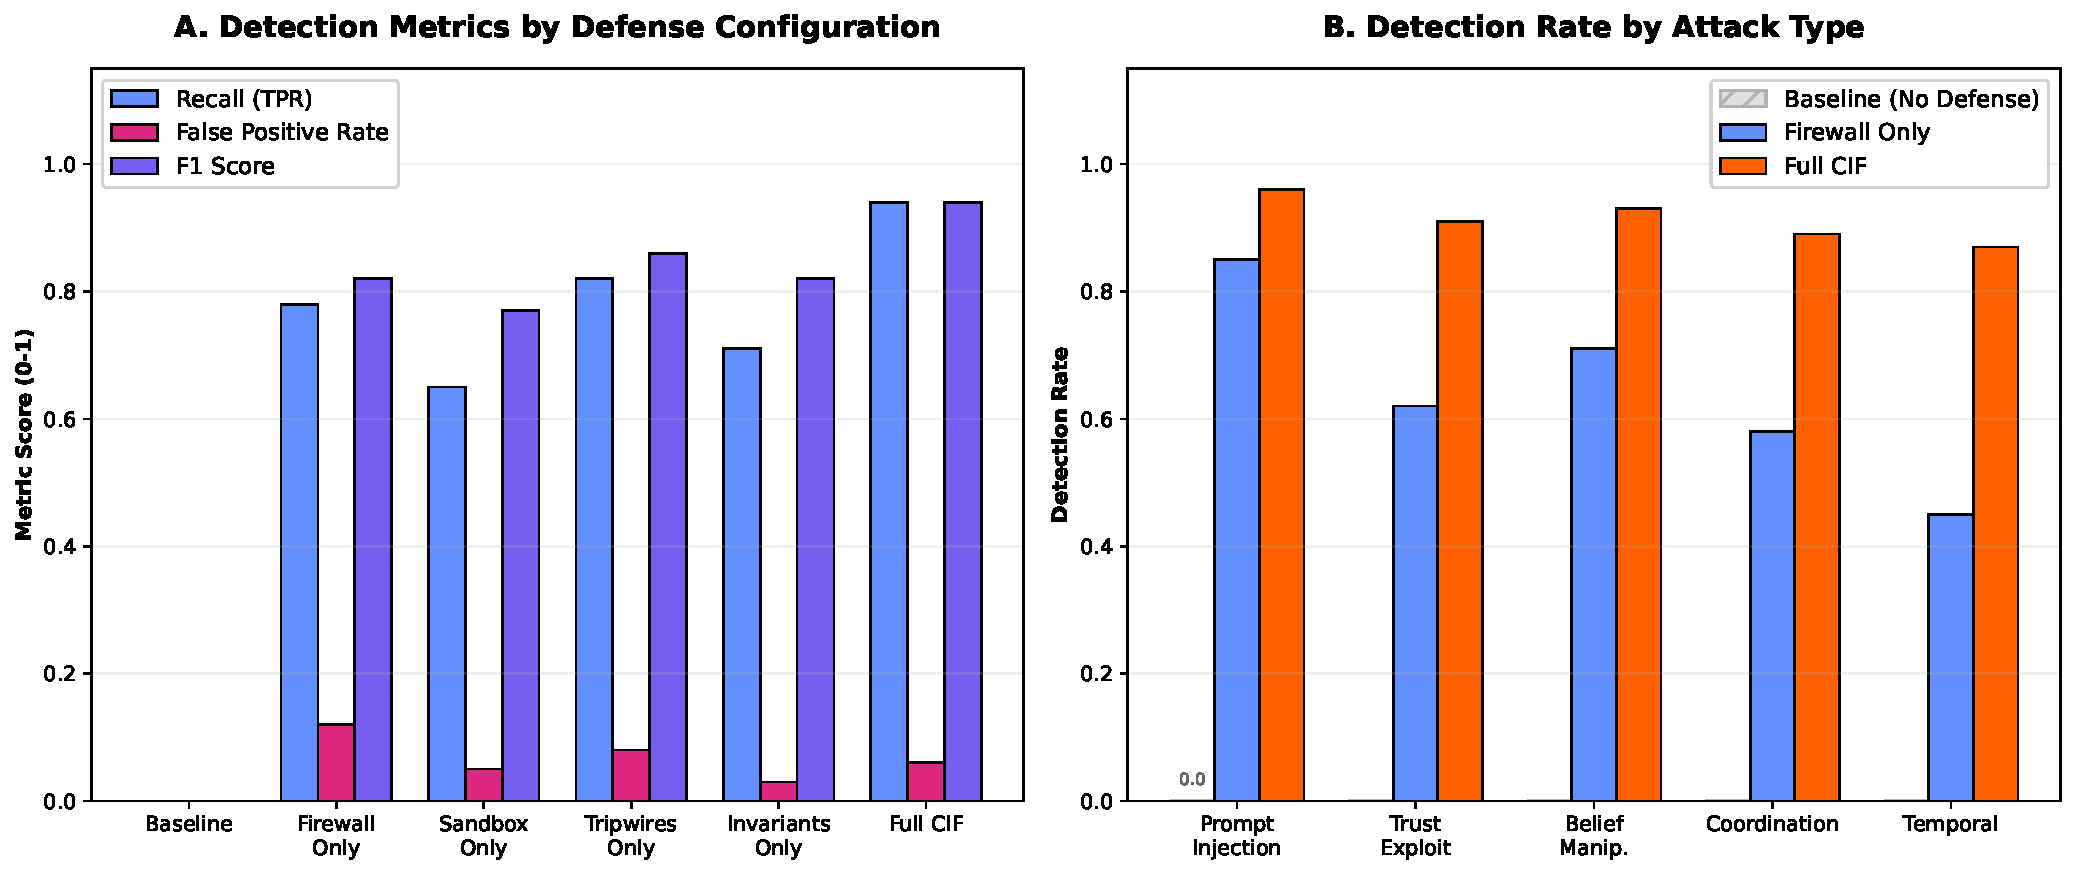
\includegraphics[width=0.85\linewidth,height=0.40\textheight,keepaspectratio,alt={Schematic detection-performance curves (illustrative, theory-guided, not measured): detection rate by attack category across representative defense stages. Measured pipeline results are reported in Part 2.}]{../figures/detection_performance.pdf}
\caption{Schematic detection-performance curves (illustrative,
theory-guided, not measured): detection rate by attack category across
representative defense stages. Measured pipeline results are reported in
Part 2.}\label{fig:detection-performance}
\end{figure}

\end{frame}

\begin{frame}[allowframebreaks]{Multi-Stage Detection Pipeline}
\emph{Real systems cannot run all detectors on all messages
simultaneously. This section formalizes a staged pipeline that applies
computationally cheap detectors first, escalating to expensive detectors
only when lower stages trigger.}
\end{frame}

\begin{frame}[allowframebreaks]{Pipeline Architecture}
\protect\phantomsection\label{pipeline-architecture}
\begin{definition}[Multi-Stage Detection Pipeline]
\label{def:multi-stage}
A $k$-stage detection pipeline is a sequence of detectors with increasing accuracy and cost:
\begin{equation}
\label{eq:pipeline}
\text{Pipeline} = (\mathcal{D}_1, \mathcal{D}_2, \ldots, \mathcal{D}_k)
\end{equation}
with \textbf{escalation rule}: message $m$ advances to stage $i+1$ if and only if $\mathcal{D}_i(m) \geq \theta_i$ (above suspicion threshold).
\end{definition}

\end{frame}

\begin{frame}[allowframebreaks]{Pipeline Architecture}
\begin{table}[htbp]
\centering
\caption{Recommended multi-stage detection pipeline configuration.}
\label{tab:pipeline-stages}
\begin{tabular}{@{}lllllp{3cm}@{}}
\toprule
Stage & Detector & Threshold & Cost & TPR & Escalation condition \\
\midrule
1 & Pattern matching & $\theta_1 = 0.3$ & 1ms & 0.75 & Pattern score $> \theta_1$ \\
2 & Semantic embedding & $\theta_2 = 0.5$ & 10ms & 0.85 & Embedding distance $> \theta_2$ \\
3 & Belief consistency & $\theta_3 = 0.4$ & 5ms & 0.80 & Consistency violation \\
4 & Trust graph analysis & $\theta_4 = 0.6$ & 20ms & 0.88 & Trust anomaly \\
5 & Ensemble fusion & $\theta_5 = 0.7$ & 50ms & 0.94 & Final decision \\
\bottomrule
\end{tabular}
\end{table}

\begin{theorem}[Pipeline Efficiency Bound]
\label{thm:pipeline-efficiency}
For a $k$-stage pipeline where fraction $\rho_i$ of messages escalate to stage $i+1$:
\begin{equation}
\label{eq:pipeline-cost}
\mathbb{E}[\text{cost per message}] = \sum_{i=1}^{k} c_i \prod_{j=1}^{i-1} \rho_j
\end{equation}
For typical values ($\rho_i \approx 0.15$ per stage), this achieves near-full accuracy at $\approx 15\%$ of the cost of running all stages on all messages.
\end{theorem}

\begin{proof}
Expected cost is the sum over stages of stage cost times probability of reaching that stage. The probability of reaching stage $i$ is $\prod_{j=1}^{i-1} \rho_j$ by the Markov property of the escalation chain.
\end{proof}

\end{frame}

\begin{frame}[allowframebreaks]{Pipeline Architecture}
\begin{theorem}[Pipeline TPR Bound]
\label{thm:pipeline-tpr}
The pipeline's overall TPR is:
\begin{equation}
\label{eq:pipeline-tpr}
\text{TPR}_{\text{pipeline}} = 1 - \prod_{i=1}^{k}(1 - \text{TPR}_i \cdot P(\text{attack reaches stage } i))
\end{equation}
Since attacks are more likely to escalate than benign messages ($\rho_i^{\text{attack}} > \rho_i^{\text{benign}}$), the pipeline is biased toward detecting attacks.
\end{theorem}
\end{frame}

\begin{frame}[allowframebreaks]{Adaptive Threshold Selection}
\protect\phantomsection\label{adaptive-threshold-selection}
\begin{definition}[Adaptive Threshold]
\label{def:adaptive-threshold}
Thresholds adapt to observed attack frequency via online Bayesian update:
\begin{equation}
\label{eq:adaptive-threshold}
\theta_i^{t+1} = \theta_i^t - \alpha_{\text{lr}} \cdot \nabla_{\theta_i} \left[C_{\text{FN}} \cdot \text{FNR}(\theta_i^t) + C_{\text{FP}} \cdot \text{FPR}(\theta_i^t)\right]
\end{equation}
where $\alpha_{\text{lr}}$ is the learning rate and $C_{\text{FN}}, C_{\text{FP}}$ are cost weights.
\end{definition}

\end{frame}

\begin{frame}[allowframebreaks]{Adaptive Threshold Selection}
This adaptive mechanism allows the pipeline to respond to shifting
attack distributions, reducing the staleness problem that affects static
threshold configurations.

\begin{quote}
\textbf{Empirical validation of this section's theory}: The detection
methods formalized here are empirically evaluated in Part 2
\cite{friedman2026cogsec2}. Key findings: (1) the multi-stage pipeline
shows biased escalation consistent with \cref{thm:pipeline-tpr}; (2)
adversarial training across five rounds demonstrates adaptive threshold
adjustment consistent with \cref{def:adaptive-threshold}, raising
hardened detection from 52.0\% at Round 1 to 67.9\% at Round 5 in Part
2's closed-form design model; (3) per-stage miss rates attributed to
\(\Omega_3\)--\(\Omega_5\) adversary classes explain the residual
detection gap between the parametric ceiling and prototype performance
(Part 2, §5g, §S08).
\end{quote}
\end{frame}

\end{document}
